

\section{Performance measures}
In aiding the quantification of the two proposed control measures, a Fitts' law test will be used. A general Fitts' law test incorporates five different performance metrics in the evaluation of movement.\cite{Kamavuako2014,Scheme2013} The five metrics and their description can be found in table \ref{fig:Fitts}    

  \begin{figure}[H]                                         
  	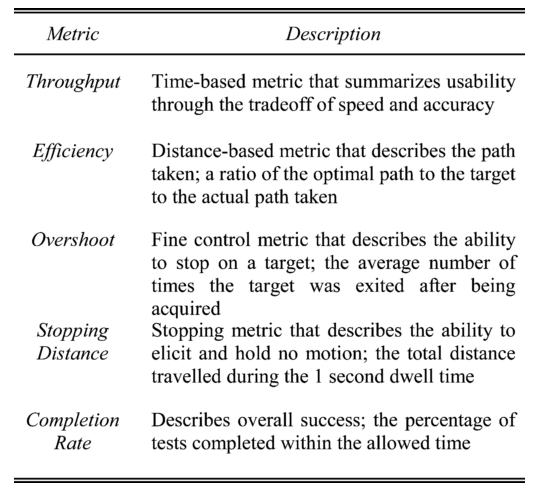
\includegraphics[width=.4\textwidth]{figures/Fitt}  
  	\caption{The table shows the metrics used in a generel Fitts' law test followed by a description of these.\cite{Scheme2013}}
  	\label{fig:Fitts} 
  \end{figure}

Often the throughput (TP) is used a single statistic representing the tradeoff between speed and accuracy. TP uses the relationship of time taken to reach a certain target in seconds (MT)   

\cite{Scheme2013} 

Put in figure of the GUI used for testing where we represent the number of targets and the distance to them. 

 